\chapter{Implementation}\label{ch:D}
\section{Development process}\label{devprc}
\begin{figure}[ht]\label{fig:market}
  \centering
  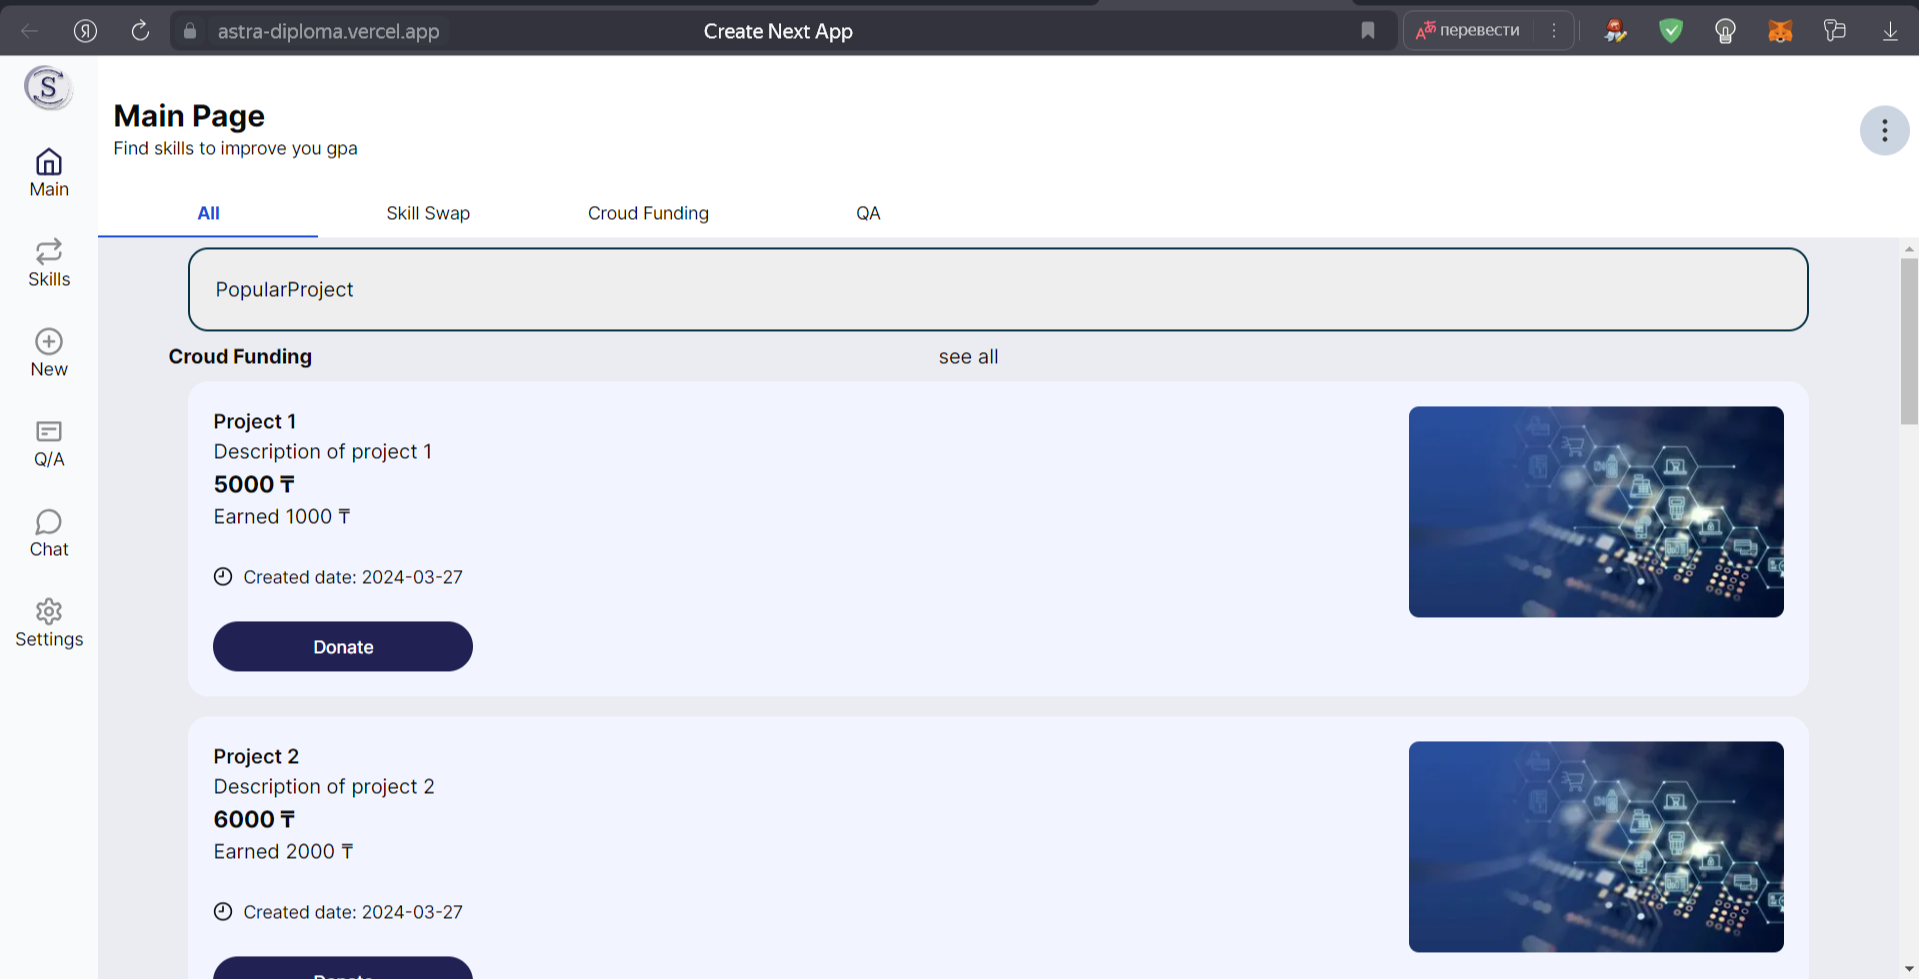
\includegraphics[width=0.8\linewidth]{figures/Website.png}
  \caption{The screenshot our website hosting on AWS \cite{aws}.}
\end{figure}

\hspace*{1cm} During the development of our products based on the mutually beneficial exchange of skills and not only this project was divided into some component parts: the \nameref{des} development process starting with wire-frames, pumping the main application design further UX/UI, the process of website design is underway to compile the visual part of the site for mobile adaptation \nameref{front}, beautiful animation, for better interaction on the website, further work is underway on \nameref{back} part is the development of functions for the operation of the site, and this is our registration form, login, chat, rating, user setup, responding to different skills, donation system search process, filters, sorting and much more and the most important deployment of the web hosting project on Amazon Web Service \cite{aws} \nameref{back} is also an \nameref{ios} - based application for mobile phones using the web view function as similar to its analogues kaspi.kz \cite{kaspi}. Let us take a closer look at every aspect of this project, namely web \nameref{des}, mobile development \nameref{ios}, and \nameref{qa} of this product writing test cases, as well as all screenshots the links will be attached below this document in -  \nameref{app:AA}.

\newpage
\section{User Flow}\label{usrflow}
\hspace*{1cm} Our user flow show \cite{miro} that the simple steps that the user performs in our application.
The purpose of this user flow \cite{miro} is to give users the opportunity to use our SkillSwap \cite{skillswap} platform in the most effective way.
\begin{itemize}
    \item \textbf{Here is the step-by-step process:}

\item The user goes to the main page of the application.
\item The user sees the website or application of the homepage where it is shared on skilswap, question answer crowd funding.
\item In order to use the platform, the user must register on the website in order to use the platform by choosing a student or an ordinary user.
\item After registration, the user can use the platform if the student all sections are available since this is a student-only platform. If a regular user, then only crowd funding is available.
\item The user can chat, ask questions, answer them, and so on. 
\item There are also settings where he can configure what number, mail, and so on he wants. 
Branching paths:
\item \textbf{Invalid email address:}
\item If the format of the email address is incorrect, an error message is displayed.
The user is prompted to enter a valid email address.
\end{itemize}

\begin{figure}[ht]\label{fig:userflow1}
  \centering
  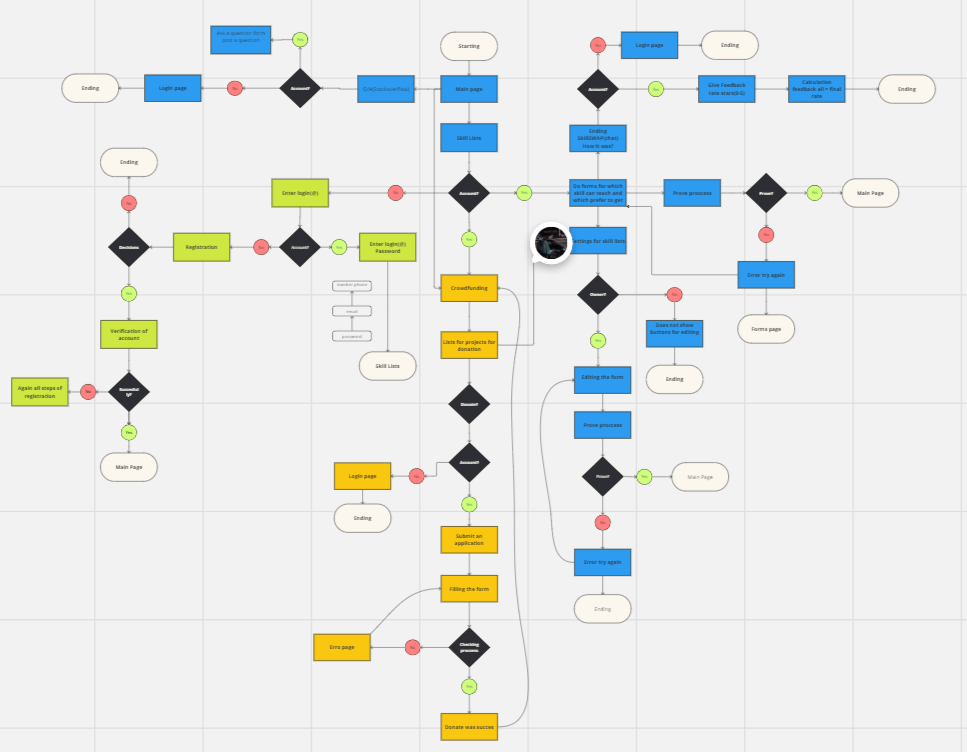
\includegraphics[width=0.8\linewidth]{figures/Userflow - 1.png}
  \caption{First type of userflow.}
\end{figure}

\begin{figure}[ht]\label{fig:userflow2}
  \centering
  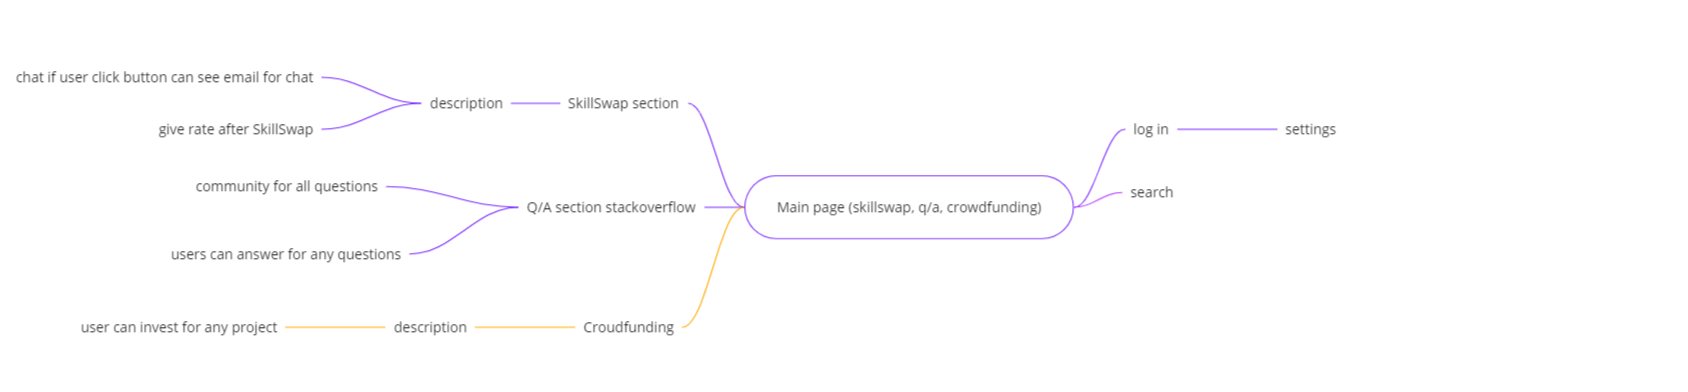
\includegraphics[width=0.8\linewidth]{figures/Userflow -2.png}
  \caption{Second type of userflow.}
\end{figure}

\newpage
\section{Implementation}\label{impl}
\subsection{Design}\label{des}
\hspace*{1cm} When brainstorming ideas about the \nameref{des} of our project, we concluded that we wanted to keep it simple, modern, and easy for users to navigate. So, we reached two main conclusions: choosing the right color to represent the entire project and prioritizing User Experience (UX) \cite{design} components. First, we defined the placement of buttons, how to display warnings, etc., to ensure a meaningful and relevant experience for users. Then, I created a wireframe \cite{wireframe}, which underwent several changes after each meeting with the team and with every new functionality change in our project.

\begin{figure}[ht]\label{fig:wireframe}
  \centering
  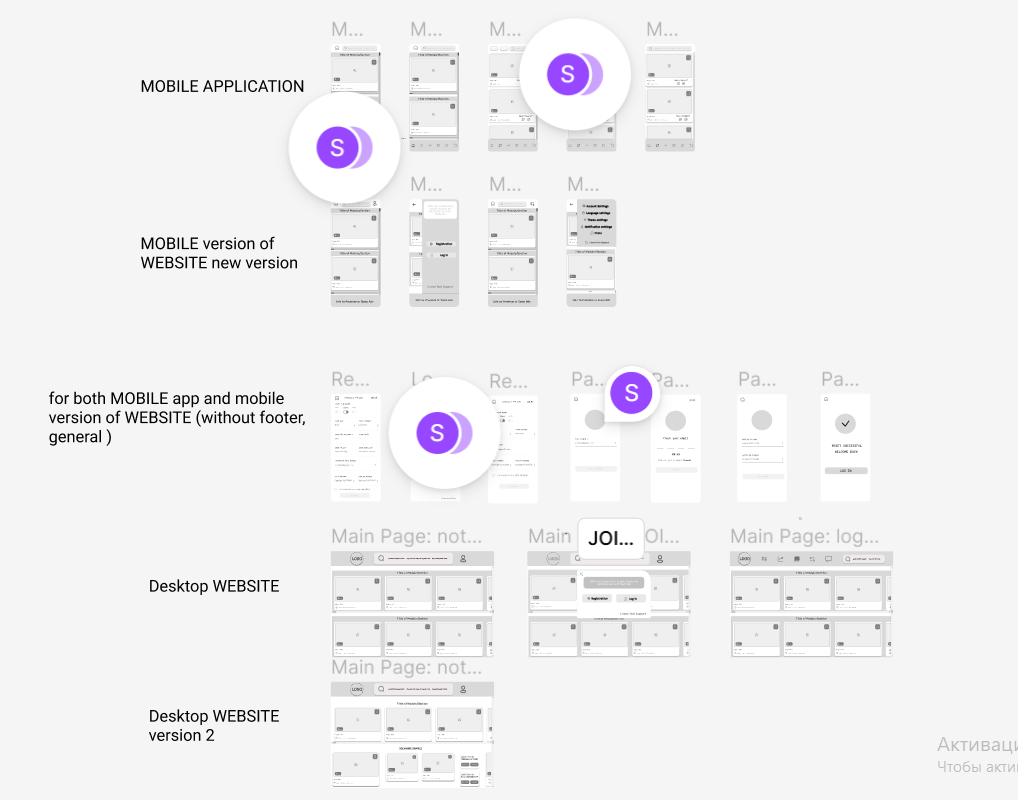
\includegraphics[width=0.8\linewidth]{figures/wireframe.png}
  \caption{The screenshot of our wireframe.}
\end{figure}
The most significant aspect for us was choosing the main color of our platform. Since our project is directly related to students, we were inspired by the representative color of our university, which is Dark Sapphire \textit{(082673)}. As we associate the university's color with tradition and honor, we decided to retain it and introduce innovation by incorporating a darker shade, resulting in Space Cadet \textit{(212153)} as our primary color. 

\begin{figure}[ht]\label{fig:colors}
  \centering
  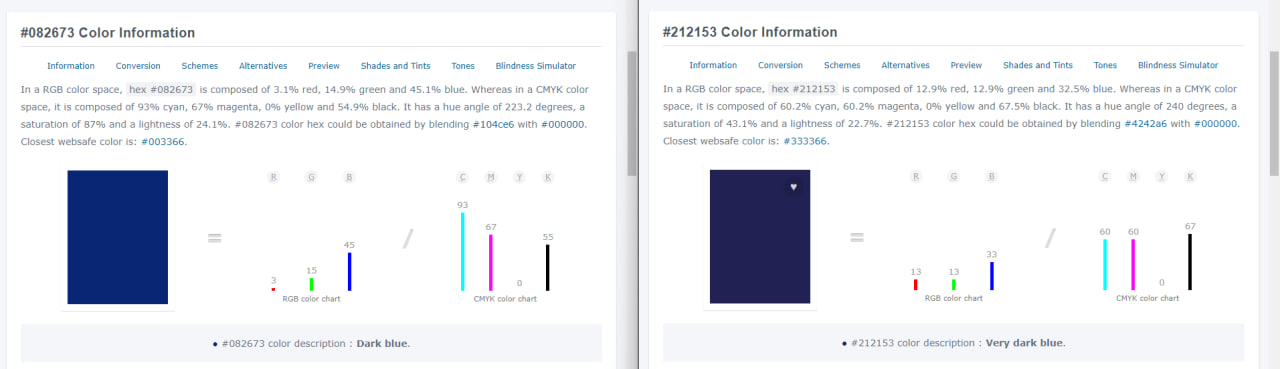
\includegraphics[width=0.8\linewidth]{figures/color comparison.jpg}
  \caption{The screenshot of comparison: University color, our project's color .}
\end{figure}
\newpage
Other colors in our project were chosen to be simple derivatives of the main color, along with gray, white, and black to maintain a classic appearance. As a result, we have achieved a \textit{minimalistic and comfortable} platform for future users.

\subsection{Frameworks}\label{frmw}
\hspace*{1cm} Decision to make Laravel \cite{laravel} the main framework for this project because of several advantages it offers. Firstly, Laravel \cite{laravel} is popular for its efficiency, what makes it perfect fit for small or medium sized web-applications, which is well-suited for our project requirements. One of the best advantages of the framework is robust debugging tool and many good libraries, which helps a lot during developing process and efficient issue resolution.
Routing system. Laravel \cite{laravel} has good and simple routing system, it simplifies the maintaining of applications routes and enhances overall code readability.Large community. Laravel \cite{laravel} has a large and active community, which proves invaluable when faced with complex challenges during development
Overall, Laravel \cite{laravel} current state as one of the most used and maintained framework ensures continuous support, regular updates, and security patches, contributing to the long-term stability and reliability of our project.
\par

\hrulefill 

To work on  \nameref{ios} we used a UI framework provided by apple themselves in 2019 - SWIFT UI \cite{swift}, which allows you to create dynamic and beautiful user interfaces with minimal effort. 

\textbf{Creating views} - We defined different views using Swift UI \cite{swift} declarative approach. Each view constitutes a separate component of the interface and can be easily adapted and reused.

\textbf{Modular architecture} - We have broken the application into small modules, each containing a set of views and functions for specific functionality. This makes the code more readable and maintainable.
For example, the screenshot below clearly shows us that we separated the UI element in the form of a sheet and built it separately so that the code would be cleaner and clearer in the whole file.

\begin{figure}[ht]\label{fig:screenios}
  \centering
  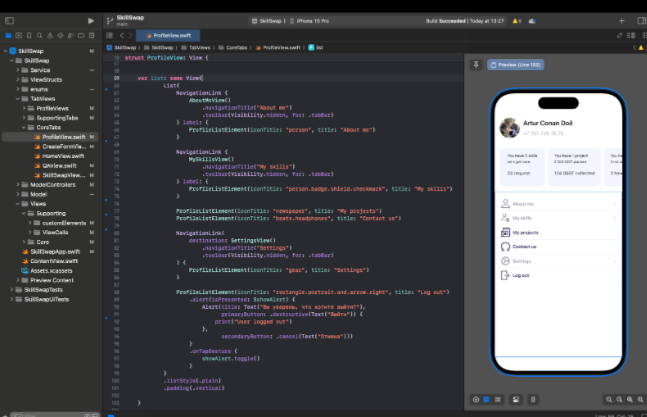
\includegraphics[width=0.8\linewidth]{figures/Screen IOS.png}
  \caption{The screenshot of our IOS application.}
\end{figure}

\subsection{Front-tend}\label{front}

\hspace*{1cm} For the React framework \cite{react}, we chose it as the main \nameref{front} \cite{htmlcssjs} framework for several reasons. \textbf{Firstly}, React \cite{react} is renowned for its efficiency, making it an ideal choice for developing small - to medium-sized web applications, which aligns perfectly with the scope of our project. Additionally, React \cite{react} boasts a powerful debugging tool and a vast array of libraries, facilitating smoother development processes and quicker issue resolution.
React \cite{react} component-based architecture offers a streamlined approach to building user interfaces, promoting code reusability and enhancing maintainability. This modular structure simplifies the development of complex applications by breaking them down into manageable components.
Furthermore, React \cite{react} benefits from a large and vibrant community of developers who actively contribute to its ecosystem. This extensive community support provides invaluable resources, including tutorials, documentation, and third-party libraries, which expedite development and troubleshooting processes. \textbf{Lastly}, React \cite{react} status as one of the most widely used \nameref{front} frameworks ensures continuous updates, feature enhancements, and security patches, bolstering the long-term stability and reliability of our project.

\subsection{Back-end}\label{back}
\hspace*{1cm} During the development of the \nameref{back} of our web application, we prioritized the adherence to the Object-Oriented Principles (OOP), including reusability, inheritance, and encapsulation. We also followed the SOLID principles, which guided our design decisions throughout the development process. Specifically, we focused on: Single Responsibility Principle: Each class or module had a single responsibility, promoting code maintainability and reducing coupling between components.
Open/Closed principle: Our code was designed to be open for extension but closed for modification, allowing for future enhancements without altering existing code.
Dependency Injection: We utilized dependency injection to invert the control of dependencies, making our code more modular, testable, and flexible.
Additionally, we aimed to keep our code DRY (Don't Repeat Yourself) \cite{dry} and KISS (Keep It Simple, Stupid) \cite{kiss}. By avoiding code duplication and complexity, we improved readability, maintainability, and debugging efficiency. In terms of design patterns, we leveraged middle ware, inspired by the Chain of Responsibility pattern, to handle common cross-cutting concerns such as authentication, logging, and request/response manipulation. Of course, the above patterns and rules we also used for our project abstractly and we tried our best to keep them.

\newpage
\subsection{Models}\label{modls}
\hspace*{1cm} Data models are created to work with the API, to transform the data we receive into a form that is understandable for our app. On \nameref{ios}, we use four main types of models:
\begin{enumerate}
    \item \textit{Authorization models} - represent the data required for the user authentication process in an application. In our application, we use two models for this purpose: 
    \item \textit{Registration model} - contains the data required to register a new user such as email, password and other required attributes. Authorization model: contains the data required for registered users to log in to the system, such as email and password.
    \item \textit{Skills Sharing Model} -  The skill sharing model represents data related to the ability of users to share their skills and services within the application. This model contains information about the user offering their skill and the user looking for the corresponding skill.
    \item \textit{Crowdfunding model} - The crowdfunding model contains data about projects that require funding from the user community. This model includes information about the project, its goals, timeline, amount of funds needed, and current fundraising status.
    \item \textit{Question and Answer (QA) Model} - the QA model is used to represent information about the questions asked by users and their corresponding answers within our application. This model contains the text of the question, a list of answers, and metadata such as the date the question was created and the number of views. This all screenshot in below in \nameref{app:BB} part
\end{enumerate}

\subsection{Views}\label{views}
\hspace*{1cm} In this part of our development, we utilized various \nameref{front} tools to create an engaging and dynamic user experience: React \cite{react} Components: Our \nameref{front} is built using React \cite{react} components, which provide a modular and reusable approach to building user interfaces. Additionally, React \cite{react} enables us to create interactive and responsive user interfaces, with data being dynamically updated as users interact with the application. CSS (cascading style sheets) Styling \cite{htmlcssjs}: We used CSS stylesheets to define the presentation and layout of our application's UI elements. We used CSS \cite{htmlcssjs} frameworks such as Bootstrap \cite{boostrap} to streamline the styling process and ensure consistency across our application. JavaScript \cite{htmlcssjs}: JavaScript played a crucial role in enhancing interactivity and functionality in our \nameref{front}. We utilized JavaScript libraries and frameworks like Axios to make asynchronous HTTP requests to our \nameref{back} API. This enabled us to retrieve and update data from the server without reloading the entire page, resulting in a smoother and more seamless user experience.

\par
\hrulefill 

Our \nameref{ios} application consists of several blocks such as:
\begin{itemize}
    \item \textit{Welcome Screen} - The Welcome Screen is where users are greeted with a brief description of our application's functionality. This screen, like a curtain, is a business card that gives a fleeting glimpse of how our application can be used.
    \item \textit{Registration Screen} - After first launching the app, users are taken to the registration screen where they can create their unique account. This step allows users to access all of the app's features, opening up a world of new possibilities.
    \item \textit{Authorization Screen} - For registered users, an authorization screen is available where they can log into their account using pre-created credentials. This step provides quick and secure access to the personal account and personalized features.
    \item \textit{MainTabView} - The Home screen is the control center for all major functions of the application. It provides a navigation hub through which users can freely navigate through the different sections of the app. Here are some of the key SubViews and HomeView: This section gives the user access to current news, updates and interesting events within the application.
    \item \textit{Skill Sharing (SkillSwapView)}: This is where users can find other users to share skills, services and knowledge.
    \item \textit{Create Post View:} This section allows users to create and publish their own posts and share information and ideas with the community.
    \item \textit{QA (QAView)}: Here users can ask questions and get answers from other community members, enriching their knowledge and experience.
    \item \textit{Profile View:} This section allows users to manage their profile, customize settings, and view their activity in the app.
    \item \textit{The MainTabView} is the main hub of user interaction with our application, providing many opportunities for users to explore, communicate, and learn.
\end{itemize}

\subsection{Forms}\label{forms}
\begin{enumerate}
    \item \textbf{Registration Purpose: Register new users to access the application functionality.}
\begin{itemize}
    \item Form fields:
    \item Email
    \item Phone number
    \item First Name
    \item Last name
    \item Password
\end{itemize}
\textbf{Actions:} Once the form is filled out, the user's data is saved in the database and the user is able to log in using their credentials.

\par
\vspace{0.5cm}

\item \textbf{Authorization Purpose: To confirm the user's identity for access to the personal account.}
\begin{itemize}
\item Form fields:
\item Login (email or phone number)
\item Password
\end{itemize}
\textbf{Actions:} After filling out the form, the data is checked for compliance with the data in the database, and in case of successful authentication the user gets access to the personal account.

\par
\vspace{0.5cm}

\item \textbf{Creating a post (Skill Swap)Purpose: To publish skill swap offers with other users.}
\begin{itemize}
    \item Form fields:
    \item Title
    \item Description (content)
    \item Photo (optional)
\end{itemize}
\textbf{Actions:} Once the form is filled out, the post is displayed on the platform where other users can see it and react.

\par
\vspace{0.5cm}

\item \textbf{Create a post (Crowdfund)Purpose: To raise funds for a specific project or product.}
\begin{itemize}
\item Form fields:
\item Product/project name
\item Description (content)
\item Amount raised
\item Planned amount
\item Photo (optional)
\end{itemize}
\textbf{Actions:} Once the form is filled out, the project is displayed on the platform where other users can see it, donate, and track fundraising progress.

\par
\vspace{0.5cm}

\item \textbf{Create a post (Question)Purpose: To ask questions and get answers from other users.}
\begin{itemize}
    \item 
Form Fields:
\item Title
\item Question (content)
\item Photo (optional)
\end{itemize}
\textbf{Actions:} After filling out the form, the question is displayed on the platform where other users can see it and leave answers.
\end{enumerate}


\subsection{IOS}\label{ios}
\hspace*{1cm}  The \nameref{ios} application gives users convenient access to your service functionality on Apple devices, allowing them to interact with the community, share skills, and create new opportunities.System Requirements: Supports \nameref{ios} version 13.0 or higher. Internet connection is also required for the app to work. Install and Run: Users can install it on their devices using the App Store or join the beta testing through TestFlight \cite{testflight}. \textit{User Interface}: The application interface is friendly and intuitive. Users can easily create posts, search for skills or ask questions using simple and straight forward controls. \textit{Application functionality:} Users can register, log in and create posts in various categories such as SkillSwap \cite{skillswap}, Crowdfund and Questions. The app provides the ability to share skills, fundraise for projects and ask questions to the community. \nameref{back} and \nameref{front} integration: The application interacts with the \nameref{back} and \nameref{front}, providing data transfer and request processing via API.

\section{Quality Assurance}\label{qa}
\hspace*{1cm} The testing process of our project began with the implementation of the \nameref{front} carcass. As the \nameref{qa}, we initiated the creation of basic UI test cases to ensure the visual correctness aligns with the approved design by our team. Once the \nameref{back} was implemented and integrated to the \nameref{front} end by our developer, It was decided to provide end-to-end testing to ensure effective validation of each functionality. Meaning of end-to-end testing is conducting tests to every possible user interaction, from registration to login and beyond, across the entirety of the platform. Subsequently, We conducted mobile testing to assess the platform's responsiveness. Finally, User Acceptance Testing (UAT) was carried out, marking the concluding phase of testing overseen by me. Additionally, routine code reviews and smoke tests were conducted by both our developers and the project manager to ensure quality and functionality

\section{Architecture}\label{arch}
\hspace*{1cm} The project is a web application designed to facilitate communication and collaboration between students, allowing them to create posts, ask questions, and participate in skill-based exchanges.
\begin{enumerate}
    \item \textbf{\nameref{front} Architecture}
\begin{itemize}
    \item The \nameref{front} of the application is built using React.js \cite{react}, a popular JavaScript \cite{htmlcssjs} library for building user interfaces.
    \item \textbf{Components:} The \nameref{front} consists of modular components that handle various aspects of the user interface, such as posts, questions, skill funds, and user profiles.
    \item \textbf{State Management:} Redux is used for state management, allowing for centralized management of application state and data flow.
    \item \textbf{Communication with \nameref{back}} : The \nameref{front} communicates with the \nameref{back} REST full API to fetch and update data using asynchronous HTTP requests.
\end{itemize}

\item \textbf{\nameref{back} Architecture}
\begin{itemize}
    \item \nameref{back} part of our web-application was written using Laravel \cite{laravel}.
    \item The \nameref{back} gives access for multiple API endpoints allowing CRUD operations for skillswaps, skillfunds and questions with their answers.
    \item Authentication and authroization is implemented by middlewares, ensuring that only authenticated users can access certain endpoints.
    \item \nameref{back} interacts with relational database (PostgreSQL) \cite{postgressql} to store information related to posts, questions, users, and their interactions.
\end{itemize}

\item \textbf{Logging}
\begin{itemize}
    \item Web-application logs every info, error and warnings into its default log system.
\end{itemize}

\item \textbf{Security}
\begin{itemize}
    \item Authorization and authentication protect application from common threats.
    \item User authorization handled by laravel \cite{laravel} sunctum, given users token for further access for our endpoints.
    \item Input validation for CRUD and other operations, prevents our application from SQL \cite{postgressql} injections.
\end{itemize}

\item \textbf{Deployment Architecture}
\begin{itemize}
    \item Application is deployed by Amazon Web Service \cite{aws}.
\end{itemize}
\end{enumerate}

\section{Databases}\label{dbms}
\hspace*{1cm} The project uses PostgreSQL \cite{postgressql} as the database management system (DBMS) \cite{dbms} due to its robust features, support for complex data types, and strong emphasis on data integrity.PostgreSQL \cite{postgressql}is an open-source RDBMS known for its reliability, extensibility, and compliance with SQL standards.
 The use of PostgreSQL \cite{postgressql} allows for the efficient storage and retrieval of structured data, enabling the application to handle large volumes of information while maintaining data consistency and reliability.
 
\begin{enumerate}
    \item \textbf{Database Schema}
\begin{itemize}
    \item The database schema is designed to reflect the application's data model, which includes entities such as users, posts, questions, skill funds, categories, and ratings.
    \item Each entity is represented by a table in the database \cite{dbms}, with columns corresponding to the entity's attributes.
    \item Relationships between entities are established using foreign key constraints, ensuring referential integrity and enforcing data consistency.
    \item The database \cite{dbms} schema is optimized for efficient querying and data retrieval, with appropriate indexing and normalization techniques applied to improve performance.
\end{itemize}

\textbf{The database \cite{dbms} schema consists of the following tables:}

\vspace{0.5cm}
\par
\item \textbf{Students Table}

\begin{itemize}
\item \textit{The students} table contains primary information about students, including their name, course, phone number, university, specialty, etc.
\end{itemize}

\item \textbf{Universities Table}
\begin{itemize}
\item \textit{The universities} table stores information about all universities in the country. It includes columns for the university's name and code.
\end{itemize}

\item \textbf{Faculties Table}
\begin{itemize}
\item \textit{The faculties} table contains information about faculties within universities. This table establishes a one-to-many relationship with universities.
\end{itemize}

\item \textbf{Specialties Table}
\begin{itemize}
\item \textit{The specialties} table holds information about all specialties offered within faculties, it establishes a one-to-many relationship with faculties.
\end{itemize}

\item \textbf{Posts Table}
\begin{itemize}
\item \textit{The posts} table allows students to create, update, and delete posts. Each post can have an associated application functionality, where students can apply for a post to buy or exchange skills. The table includes columns for description, image, title, and status.
\end{itemize}

\item \textbf{Questions Table}

\begin{itemize}
\item \textit{The questions} table enables students to create and answer questions. Each question can be rated on the basis of its quality and the students can also provide answers. The table includes columns for title, question, image, and rating.
\end{itemize}

\item \textbf{Skill Funds Table}

\begin{itemize}
\item \textit{The skill funds} table is designed for students to share their startup ideas. Students can earn money if their idea gains enough popularity and support. The table includes columns for description, title, and status.
\end{itemize}
\end{enumerate}
\textbf{Cache}

In our application, we used caching to improve performance and reduce database \cite{dbms} load. Caching helps store frequently accessed data in memory, allowing for faster retrieval and response times.
\vspace{0.5cm}
\par
\textbf{We employed caching in various parts of the application, such as:}

\begin{itemize}
    \item \textbf{Database Query Results}: We cached the results of frequently executed database queries to avoid redundant database calls and speed up data retrieval.
    
    \item \textbf{API Responses}: We cached API responses to reduce latency for subsequent requests and improve overall API performance.
    
    \item \textbf{View Fragments}: We cached rendered views or view fragments to enhance the responsiveness of the application and reduce server-side processing time.
\end{itemize}

By leveraging caching mechanisms, we were able to optimize the performance of our application and deliver a smoother user experience.

\section{Additional tools}\label{tools}
\textbf{Swagger \cite{swager}}

\begin{itemize}
\item Swagger \cite{swager} was used for providing user-friendly interface for \nameref{front} and mobile developer \nameref{ios}. Our REST API \cite{rest} endpoints was documented and visualized using this technology.
\end{itemize}

\textbf{Amazon Web Services (AWS) \cite{aws}}
\begin{itemize}
    \item  We used AWS \cite{aws} for deploying our web-application.
\end{itemize}

\begin{itemize}
\item \textbf{Amazon EC2 (Elastic Compute Cloud)}: EC2 instances allowed to host and run our application.
    
\item \textbf{Amazon Route 53}: Route 53, AWS highly available and scalable DNS web service, was used for domain registration, routing traffic to our application resources, and managing domain health checks and failover configurations. It ensured reliable and efficient DNS resolution for our web applications.
\end{itemize}

\textbf{Vercel \cite{vercel}}
\begin{itemize}
\item Vercel \cite{vercel} was used to deploy our front-end part.
\end{itemize}
\textbf{Git / Github \cite{github}}
\begin{itemize}
\item members and enabling versioning, code review, and issue tracking throughout the development process. It provided a centralized repository for our codebase, ensuring visibility, traceability, and code integrity.
\end{itemize}

\hrulefill 
\vspace{0.5cm}
\par
In our \nameref{ios} application, we have chosen the MVVM (Model-View-ViewModel) architectural pattern to organize the code. MVVM offers a solution to structure the application by dividing it into three main components: model (Model), view (View) and view model (ViewModel).Why we chose MVVM: Separation of Responsibilities: MVVM helps us to clearly separate the business logic (Model), the UI mapping (View) and the interaction logic between them (ViewModel).
\vspace{0.5cm}
\par
\textbf{Ease of testing:} By separating the code into separate components, we can easily test each part independently. The view model can be tested with unit tests without having to run the UI.
Support for multiple interfaces: MVVM makes it easy to create different user interfaces such as for mobile devices, web applications or desktop applications using the same presentation model.
\vspace{0.5cm}
\par
\textbf{Cleaner and clearer code:} MVVM facilitates the creation of clean and understandable code by clearly separating logic and display.
Support for bi-directional data binding: MVVM provides bi-directional data binding between the view and the view model, which makes the process of updating data on the UI easier and more efficient. Using MVVM allows us to create flexible, maintainable and easily testable applications, which improves development productivity and provides a better user experience.
